\chapter{Simple Template Language}
\label{Chapter: STL}

There are many template languages available. The {\em Simple Template
Language} distinct attributes are:

\begin{itemize}
  \item optimized to work with XML files\footnote{{\bf STL} is implemented
    as an XML namespace.};
  \item very easy to learn;
  \item high productivy;
  \item fast.
\end{itemize}

I like to define {\bf STL} as a {\em descriptive} language. It is amazing
how many template languages are out there that allow to put Python code
inside a template, and call it a feature.


\section{How it works}

The Figure~\ref{Figure: stl} shows how {\bf STL} works. The input for
{\bf STL} is a source template and a Python namespace, the output is
a new XML template.

\begin{figure}
  \center
  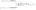
\includegraphics[width=\textwidth]{stl.eps}
  \caption{The Simple Template Language ({\bf STL})}
  \label{Figure: stl}
\end{figure}

There are solutions like htmlgen\footnote{XXX} or XX that allow to produce
the XML or HTML output enterily from Python. While with tools like
ZPT\footnote{XXX} it is possible to produce a complex web page only from
a source template.

We think it is easier to read code when it is written in Python, and it is
easier to read XML when it is written in XML. This is the reason {\bf STL}
not just allows, but enforces, the separation between logic and presentation.

The language {\bf STL} don't includes any programming constructions, the
four statements it provides only describe the transformations to be
performed on the source template.

Lets see a simple example.

\subsection{The template}

For example, look at the template below ({\tt examples/chapter9/template.xml}):

\begin{code}
    <?xml version="1.0" encoding="UTF-8"?>
    <html xmlns="http://www.w3.org/1999/xhtml"
          xmlns:stl="http://xml.itools.org/namespaces/stl">
      <head></head>
      <body>
        <h1 stl:content="title" />
      </body>
    </html>
\end{code}

Note the declaration of the {\em stl} namespace, it is mandatory since
{\bf STL} is implemented as an XML namespace.

When this template will be processed, the content of the {\tt <h1>} tag
will be replaced by the value of the variable {\tt title}. But, where will
we find {\tt title}? Solution: in the namespace.

\subsection{The namespace}

The namespace is a mapping that is built from the Python side. Then with
the template and the namespace we will just call the {\tt stl} function
to get the output. See:

\begin{code}
    >>> from itools.handlers import get_handler
    >>> from itools.xml.stl import stl
    >>>
    >>> namespace = {'title': 'hello world'}     # 1. Build the namespace
    >>> template = get_handler('template.xml')   # 2. Load the template
    >>> print stl(template, namespace)           # 3. Go!
    <?xml version="1.0" encoding="UTF-8"?>
    <html xmlns:stl="http://xml.itools.org/namespaces/stl"
          xmlns="http://www.w3.org/1999/xhtml">
      <head></head>
      <body>
        <h1>hello world</h1>
      </body>
    </html>
\end{code}

As the output shows, the value of the variable {\tt title} is looked within
the namespace.


\section{The Language}

\subsection{STL attributes}

There are four {\bf STL} attributes:

\begin{itemize}
  \item {\tt stl:content}=``{\em expression}''

    Replaces the element's
    content by the result of evaluating the given expression.

  \item {\tt stl:attributes}=``{\em name expression}[; {\em name expression}]*''

    For every pair ``{\em name: expression}'', replace the the value of
    the attribute {\em name} by the result of evaluating {\em expression}.

  \item {\tt stl:if}=``[not ]{\em expression}''

    If the given expression evaluates to {\tt True}, do nothing; if
    evaluates to {\tt False}, remove the XML element.

  \item {\tt stl:repeat}=``{\em name expression}''

    The given expression is expected to be a sequence or an iterator.
    For every item in {\em expression}, create an element and add the
    item to the namespace stack before processing the element.
\end{itemize}


\subsection{Expressions}

The {\bf STL} expressions are pretty simple, their syntax is:

\begin{quote}
    name[/name]*
\end{quote}

That is, a sequence of names separated by slashes. The semantics is:

\begin{enumerate}
  \item Look the first name in the namespace stack.

  \item If there are more names left, the last value found must be a namespace,
    then look the next name in that namespace.

    Iterate until the last name is consumed.

  \item Once the end of the sequence is reached, we will have a value. If
    the value is callable, then call it to get a new value.

  \item Finally, we should have a value that is either a string, a boolean
    or a sequence, depending on which statement ({\tt content}, {\tt repeat},
    etc.) the expression is being used with.
\end{enumerate}



\section{Example: Task Tracker}

Now we are going to illustrate {\bf STL} with a more complex example.
Building up on the Task Tracker from the Chapter~\ref{section: files2},
we are going to write a method that produces an HTML page showing all
the tasks.

First, the template (see {\tt examples/chapter9/TaskTracker\_view.xml}):

\begin{code}
    <?xml version="1.0" encoding="UTF-8"?>
    <!DOCTYPE html
         PUBLIC "-//W3C//DTD XHTML 1.0 Transitional//EN"
         "http://www.w3.org/TR/xhtml1/DTD/xhtml1-transitional.dtd">
    <html xmlns="http://www.w3.org/1999/xhtml"
          xmlns:stl="http://xml.itools.org/namespaces/stl">
      <head></head>
      <body>
        <h2>Task Tracker</h2>
        <div stl:repeat="task tasks">
          <h4>
            #<stl:block content="task/id" />:
            <stl:block content="task/title" />
            (<em stl:content="task/state" />)
          </h4>
          <p stl:content="task/description" />
        </div>
      </body>
    </html>
\end{code}

The first new thing this example shows is the {\tt repeat} statement. While
{\tt stl:content} expects a string as the value, {\tt stl:repeat} expects a
sequence. When this template is processed, the XML output will contain as
many {\tt <div>} elements as tasks are in the {\tt tasks} variable. Within
the div element, in each iteration over the {\tt tasks} sequence, the
variable {\tt task} will be the respective item of the list.

The second new thing we see is the {\tt <stl:block>} element. When the
template is processed the {\tt <stl:block>} tags are automatically
removed.

Finally, look at the expression {\tt task/id} or {\tt task/title}, it shows
the {\em slash} operator, which lets to traverse namespaces. So the variable
{\tt task} is expected to be a mapping (e.g. a dictionary), and
{\tt id} a key in that mapping, whose value is a string.

\subsubsection{The Python side}

Now let's see the Python code (see {\tt examples/chapter9/TaskTracker.py}).
Basically we have added the method {\tt view} to the class {\tt TaskTracker}:

\begin{code}
    def view(self):
        # Load the STL template
        handler = get_handler('TaskTracker_view.xml')

        # Build the namespace
        namespace = {}
        namespace['tasks'] = []
        for i, task in enumerate(self.state.tasks):
            namespace['tasks'].append({'id': i,
                                       'title': task.title,
                                       'description': task.description,
                                       'state': task.state,
                                       'is_open': task.state == 'open'})

        # Process the template and return the output
        return stl(handler, namespace)
\end{code}

To try the code run the Python interpreter and type:

\begin{code}
    >>> from itools.handlers import get_handler
    >>> import TaskTracker
    >>> 
    >>> task_tracker = get_handler('itools.tt')
    >>> print task_tracker.view()
    <?xml version="1.0" encoding="UTF-8"?>
    <!DOCTYPE html
         PUBLIC "-//W3C//DTD XHTML 1.0 Transitional//EN"
        "http://www.w3.org/TR/xhtml1/DTD/xhtml1-transitional.dtd">
    <html xmlns:stl="http://xml.itools.org/namespaces/stl"
          xmlns="http://www.w3.org/1999/xhtml">
      <head></head>
      <body>
        <h2>Task Tracker</h2>
        <div>
          <h4>
            #0:
            Re-write the chapter about writing handler classes.
            (<em>closed</em>)
          </h4>
          <p>A new chapter...
\end{code}

The Figure~\ref{Figure: task tracker} shows how the HTML looks with a
browser.

\begin{figure}
  \center
  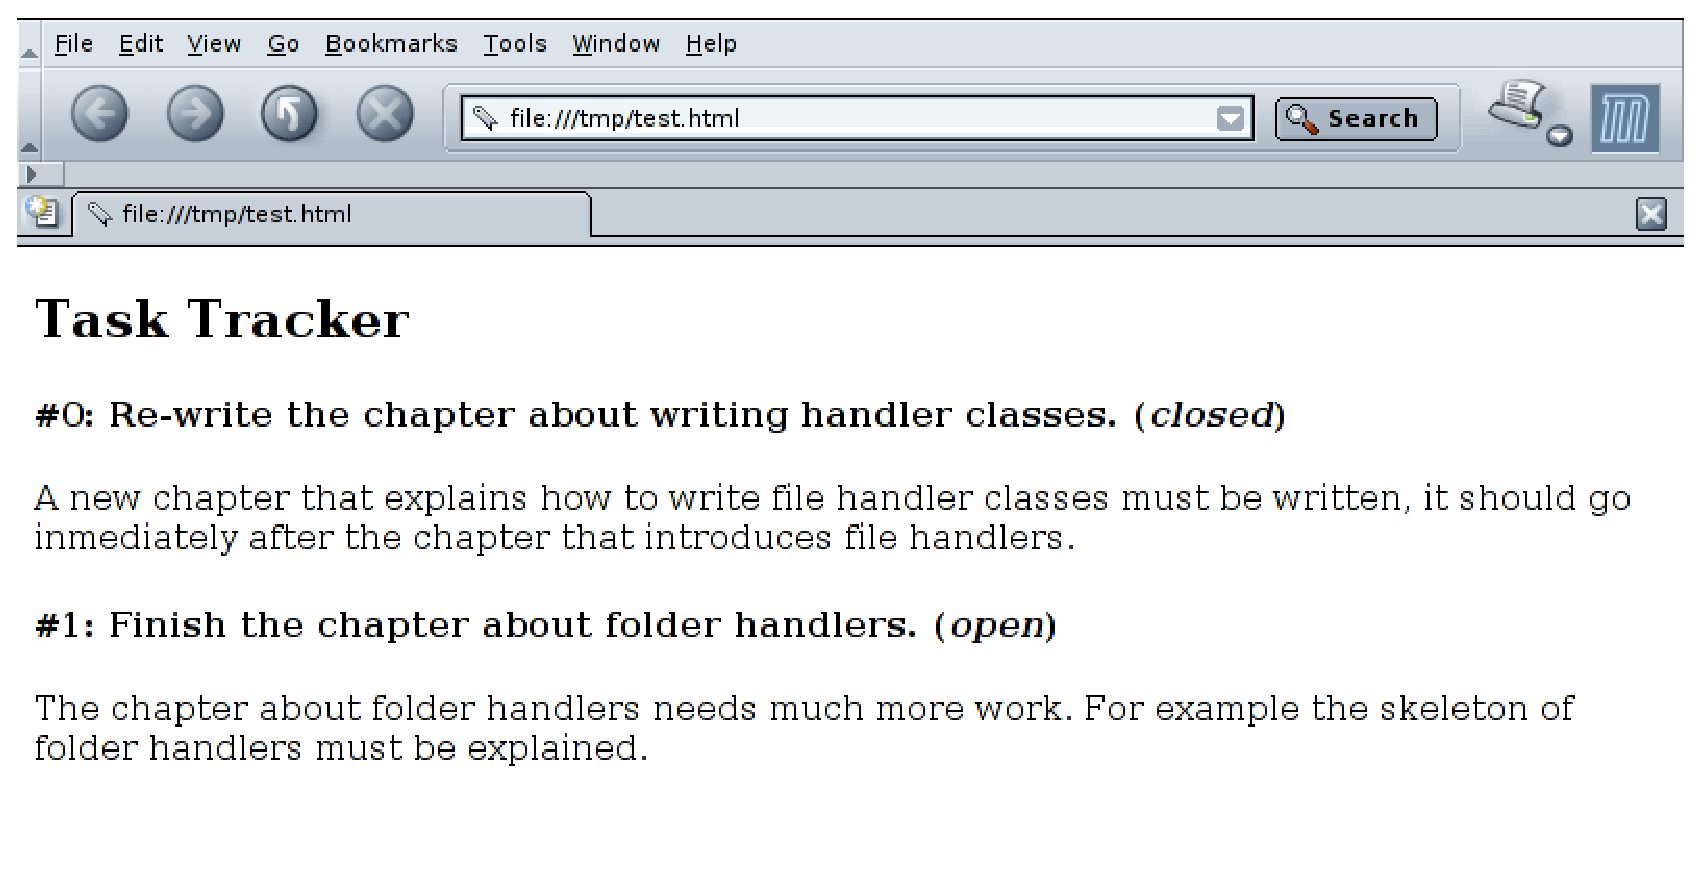
\includegraphics[width=\textwidth]{task_tracker.eps}
  \caption{The task tracker view}
  \label{Figure: task tracker}
\end{figure}

